\documentclass[10pt]{article}
\usepackage[utf8]{inputenc}
\usepackage[activeacute,spanish]{babel}
\usepackage[left=1.5cm,top=1.5cm,right=1.5cm, bottom=1.5cm,letterpaper, includeheadfoot]{geometry}

\usepackage{amssymb, amsmath, amsthm}
\usepackage{graphicx}
\usepackage{hyperref}
\usepackage{lmodern,url}
\usepackage{paralist} %util para listas compactas
\usepackage{xcolor}
\usepackage{bbm}
\usepackage{mathrsfs}
\usepackage{bbm}

%========PAQUETES AGREGADOS===========
%Pseudocodigo
\usepackage{pseudocode}
\usepackage[portuguese, boxruled]{algorithm2e}
\usepackage{wrapfig}
\usepackage{multicol}
\usepackage{graphicx}
\usepackage{caption}
\usepackage{subcaption}
%\captionsetup[table]{labelformat=empty}
\captionsetup[subfigure]{labelformat=empty}
\usepackage{cancel}
\usepackage{tikz}
\def\checkmark{\tikz\fill[scale=0.4](0,.35) -- (.25,0) -- (1,.7) -- (.25,.15) -- cycle;} 
%====================================

\usepackage{fancyhdr}
\pagestyle{fancy}
\fancypagestyle{plain}{%
\fancyhf{}
\lhead{\footnotesize\itshape\bfseries\rightmark}
\rhead{\footnotesize\itshape\bfseries\leftmark}
}


% macros
\newcommand{\Q}{\mathbb Q}
\newcommand{\R}{\mathbb R}
\newcommand{\N}{\mathbb N}
\newcommand{\Z}{\mathbb Z}
\newcommand{\C}{\mathbb C}
\newcommand{\BigO}{\mathcal{O}}
%Teoremas, Lemas, etc.
\theoremstyle{plain}
\newtheorem{teo}{Teorema}
\newtheorem{lem}{Lema}
\newtheorem{prop}{Proposición}
\newtheorem{cor}{Corolario}
\newtheorem{obs}{Observación}
\newtheorem{ej}{Ejemplo}
\renewcommand{\qedsymbol}{\rule{0.7em}{0.7em}}
\renewenvironment{proof}{{\bfseries \noindent Demostración}}{ \qed \\}


\theoremstyle{definition}
\newtheorem{defi}{Definición}
% fin macros


\newcommand{\catnum}{24} %numero de catedra
\newcommand{\fecha}{6 de Diciembre 2016 }

%%%%%%%%%%%%%%%%%%

%Macros para este documento
\newcommand{\cin}{\operatorname{cint}}



\begin{document}
%Encabezado
\fancyhead[L]{Facultad de Ciencias Físicas y Matemáticas}
\fancyhead[R]{Universidad de Chile}
\vspace*{-1.2 cm}
\begin{minipage}{0.6\textwidth}
\begin{flushleft}
\hspace*{-0.5cm}\textbf{MA3402-1 Estadística. Primavera 2016}\\
\hspace*{-0.5cm}\textbf{Profesor:} Raul Gouet\\
\hspace*{-0.5cm}\textbf{Escriba:} Manuel Cáceres\\
\hspace*{-0.5cm}\textbf{Fecha:} \fecha
\end{flushleft}
\end{minipage}
\begin{minipage}{0.36\textwidth}
\begin{flushright}

\includegraphics[scale=0.3]{imagenes/fcfm_dcc}
\end{flushright}
\end{minipage}
\bigskip
%Fin encabezado

\begin{center}
\LARGE\textbf{Clase \catnum}
\end{center}
\section{Análisis en Componentes Principales (ACP)}
Este es un método clásico (años 30 del SXX) de reducción de dimensionalidad. Reinventado 100 veces por los ``data miners''.

Veremos un procedimiento puramente descriptivo, sin probabilidad.
Solo necesitamos algo de álgebra lineal.

\section{Primeros elementos}
Sea I un conjunto de $n$ individuos (objetos). Cada uno de estos individuos está descrito por $p$ variables cuantitativas, que las denotamos $J$.\\

Digamos que el valor de la variable $j\in J$ sobre el individuo $i\in I$ es $x_{ij}$.

Se definen los vectores siguientes:
\begin{itemize}
\item $x_{i} = \begin{bmatrix}
x_{i_{1}} \\ \ldots \\ x_{i_{p}}
\end{bmatrix}\in \mathbb{R}^p = E$ (espacio de individuos), $i = 1 \ldots n$
\item $x_{j} = \begin{bmatrix}
x_{j_{1}} \\ \ldots \\ x_{j_{n}}
\end{bmatrix}\in \mathbb{R}^n = E$ (espacio de las variables), $i = 1 \ldots p$
\item La nube de individuos es el conjunto $\mathcal{M} = \{x_{i}\colon i \in I\} \subseteq E$
\item La nube de individuos es el conjunto $\mathcal{N} = \{x_{j}\colon j \in J\} \subseteq F$
\end{itemize}
\begin{center}
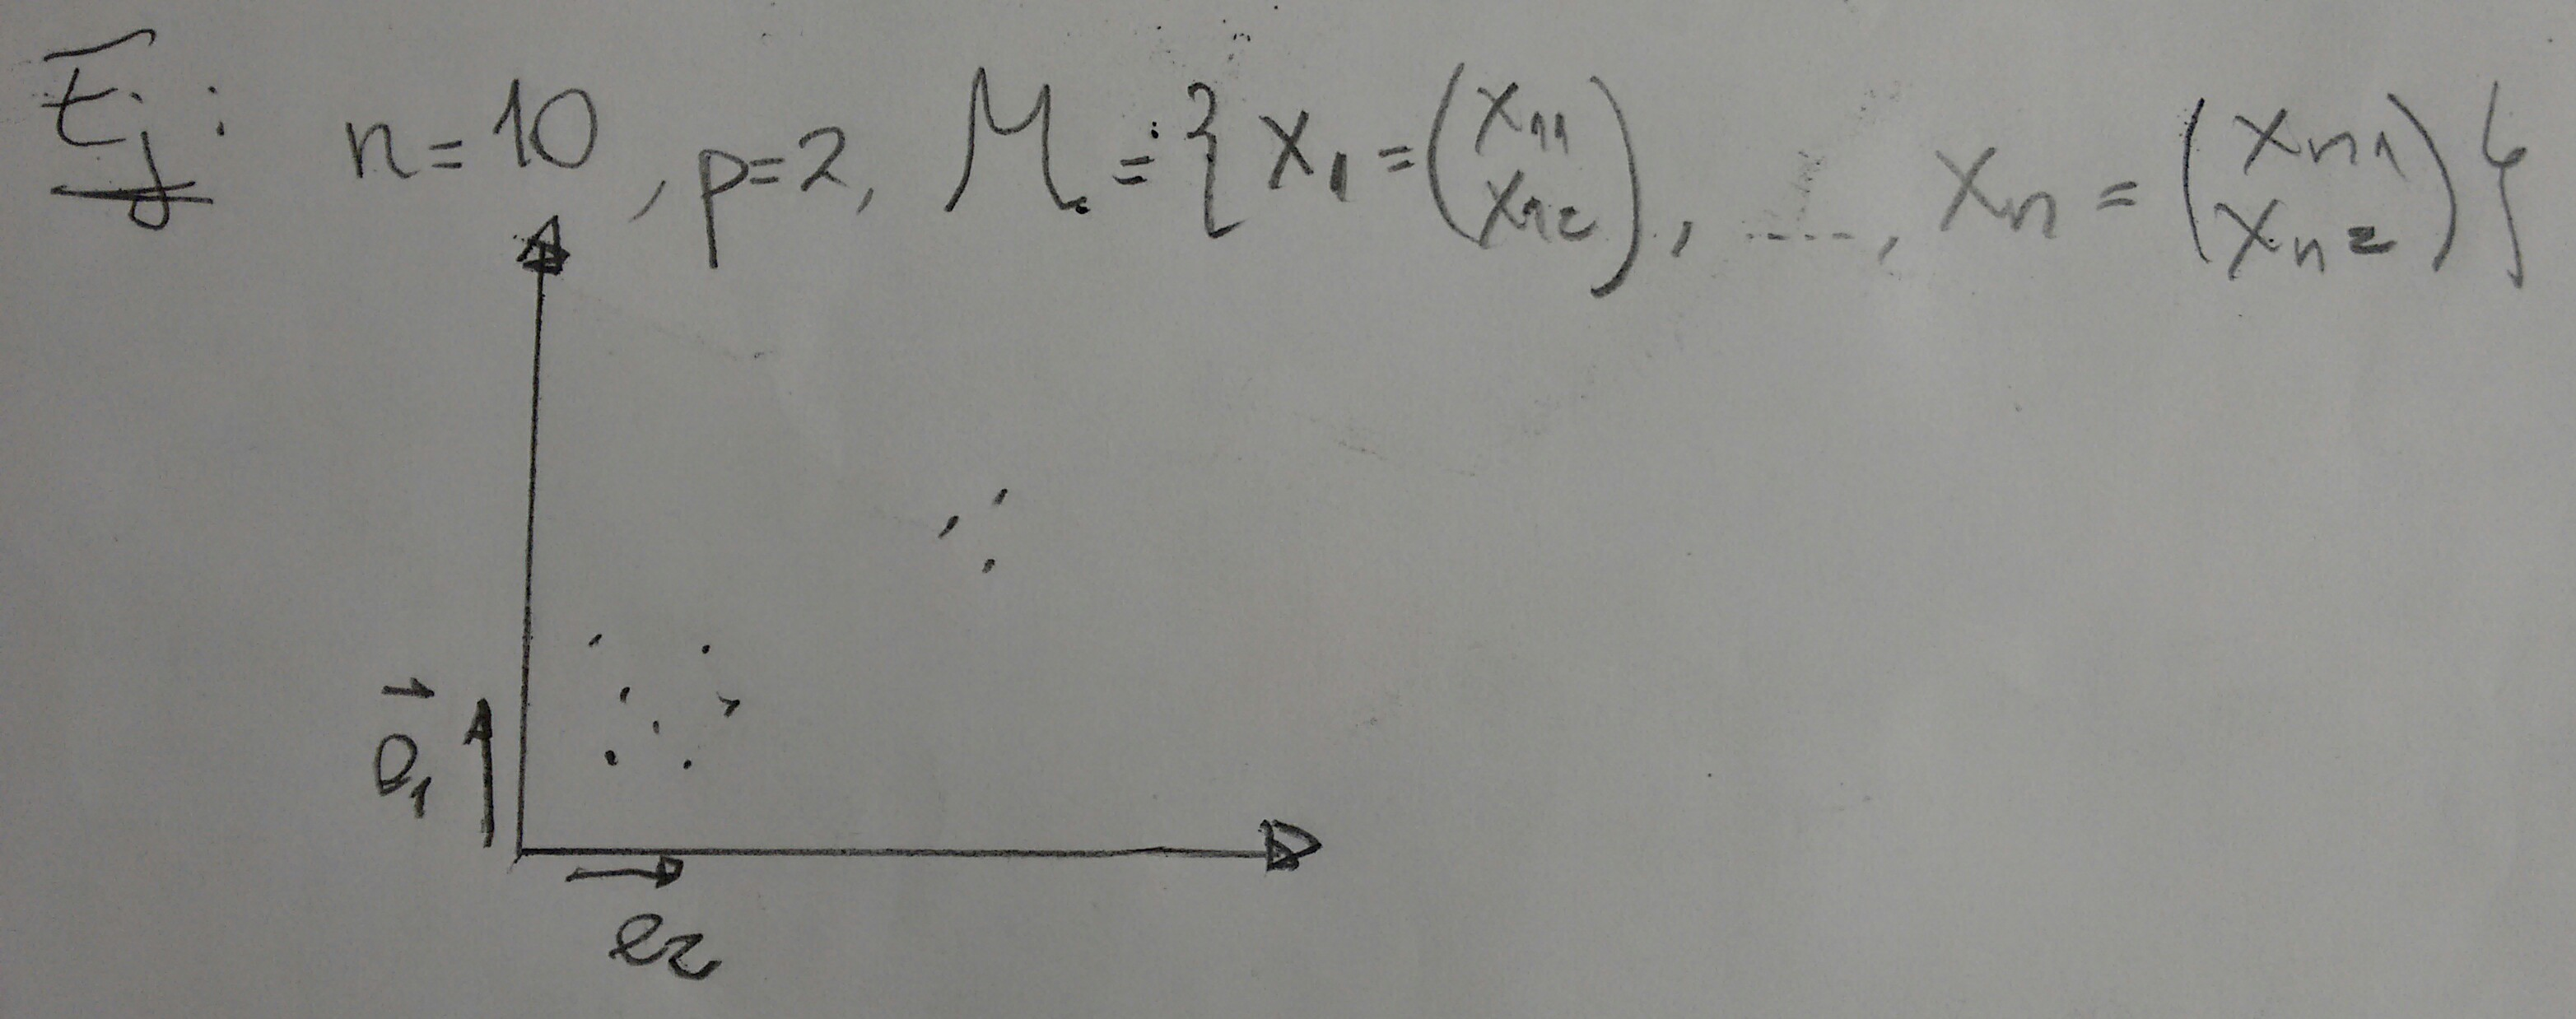
\includegraphics[scale=0.1]{imagenes/ejemplo1.jpg}
\end{center}
\begin{center}
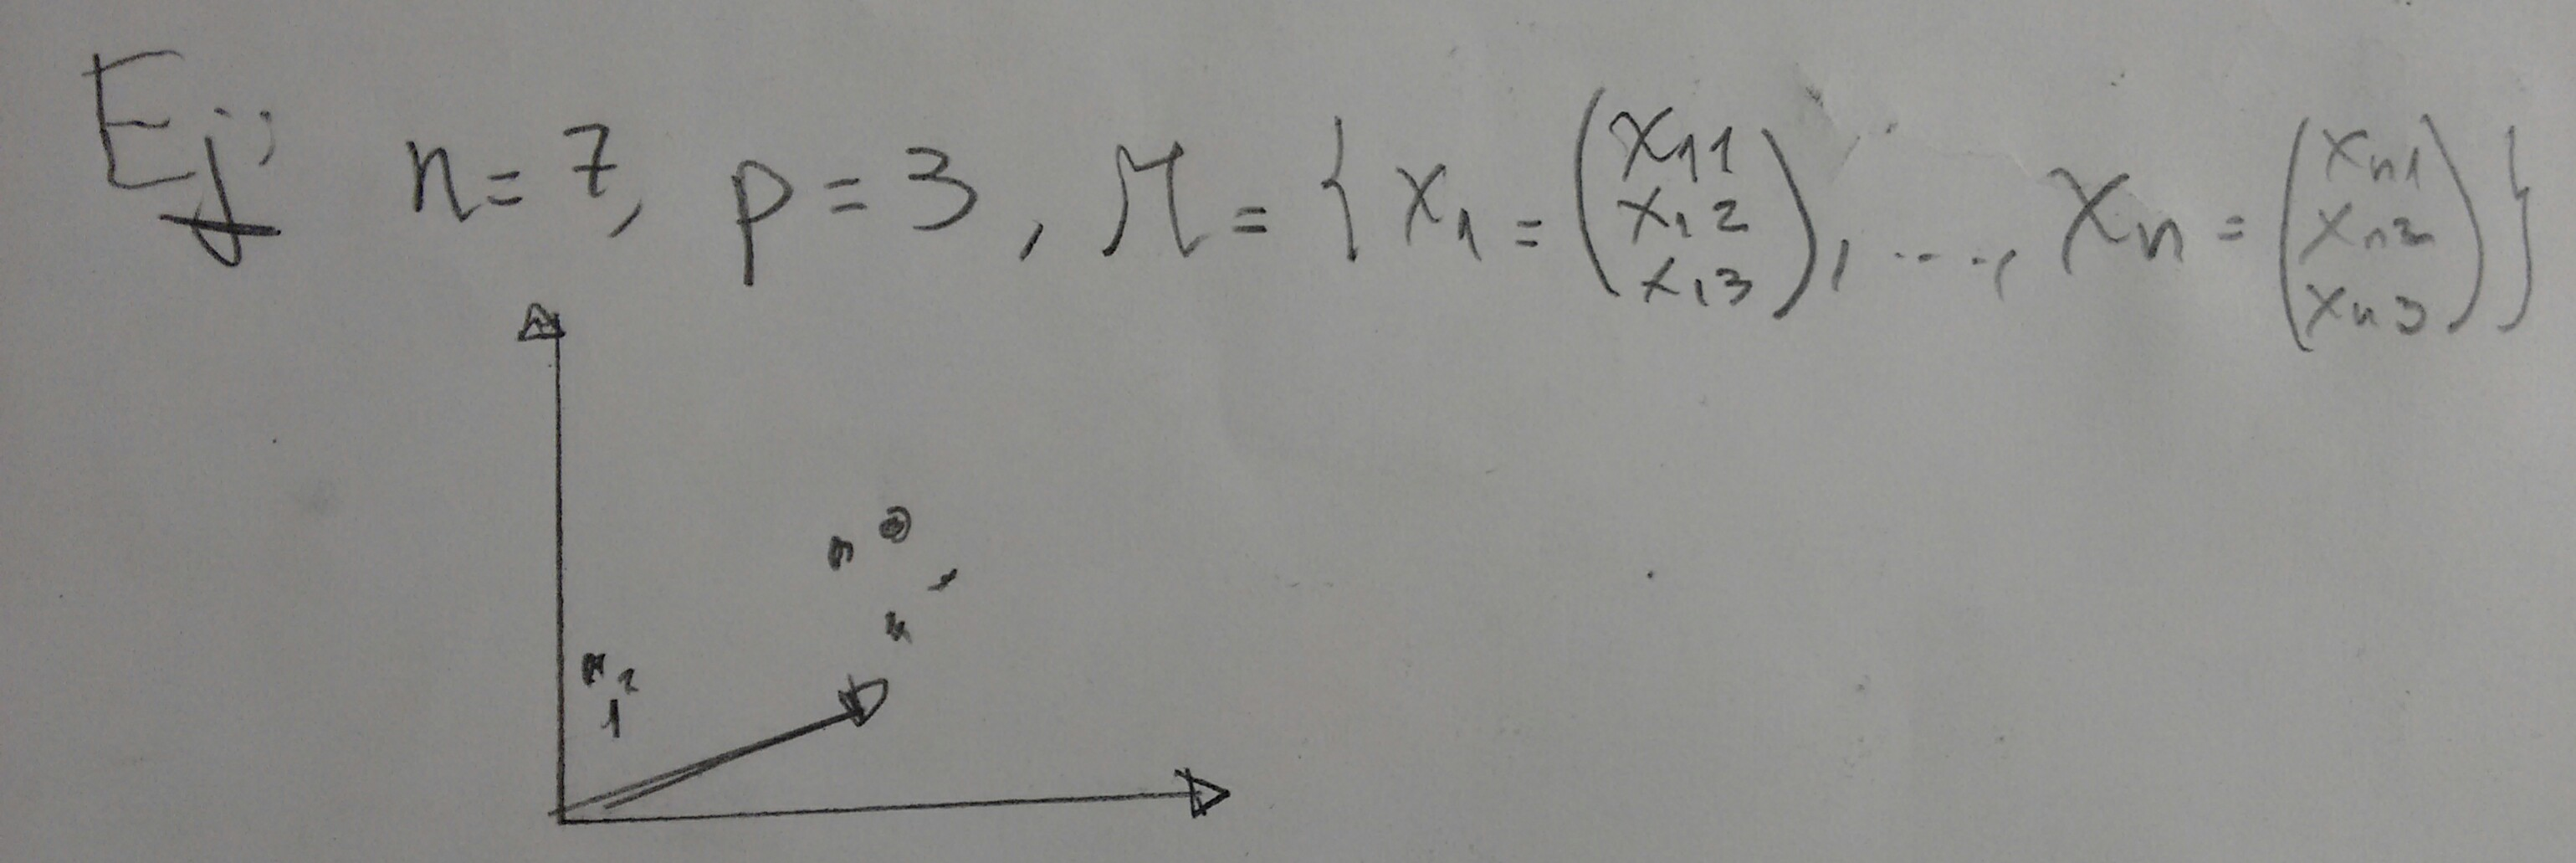
\includegraphics[scale=0.1]{imagenes/ejemplo2.jpg}
\end{center}
\section{Objetivo del ACP}
$\mathcal{M}$ vive en $\mathcal{R}^p$ y $p$ es grande en general. El ACP se propone representar a $\mathcal{M}$ en un subespacio de dimensión baja, con mínima pérdida de información (que podría ser 0).
\begin{center}
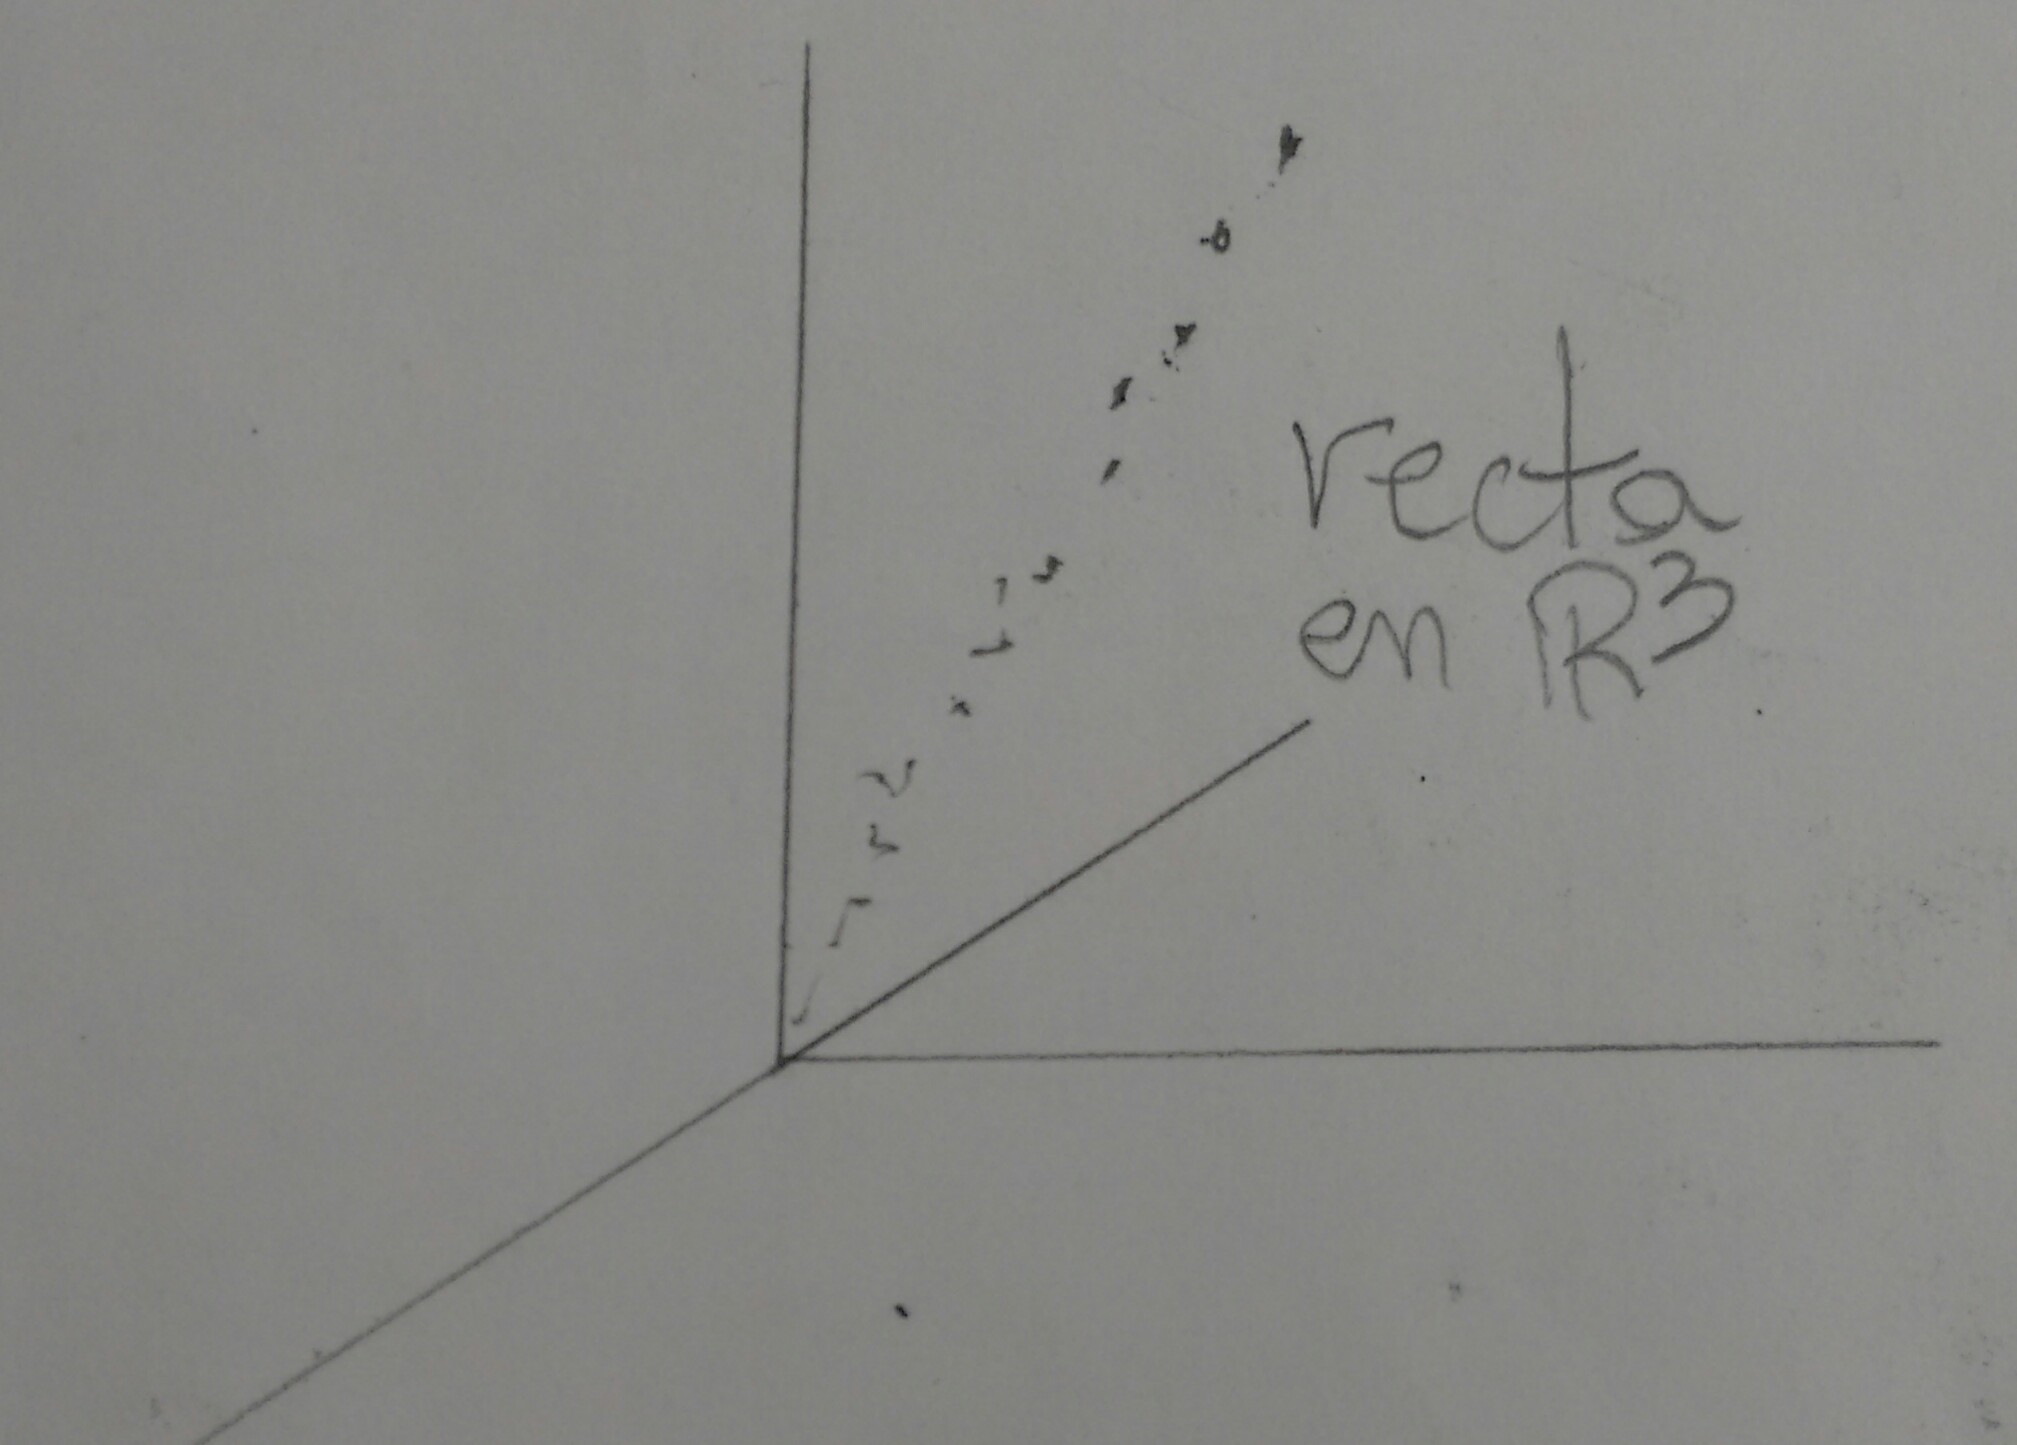
\includegraphics[scale=0.1]{imagenes/rectaenr3.jpg}
\end{center}

Esto es fácil de ver aquí, pero supongamos que p=7 y el subespacio es 3.\\

Buscamos un subespacio vectorial afín, de dimensión la dada, tal que $\mathcal{M}$ proyectada sobre este subespacio sufra mínima distorsión.\\

¿Qué es la distorsión?\\

Introducimos la idea de inercia.
Definimos inercia con respecto a un punto en E.\\

Sea $a\in E$ se define la inercia de la nube $\mathcal{M}$ con respecto a $a$ como
\begin{align*}
I_{a} = \sum_{i \in I} p_{i}||x_{i}-a||^2
\end{align*}
donde $p_{1}, \ldots, p_{n} >= 0$ son pesos asociados a los individuos, tales que $\sum_{i\in I} p_{i} = 1$. Por otra parte $||.||$ es la norma en $\mathbb{R}^p$. También usamos $<,>$ para el producto interno $<a,b> = a'b$.\\

Mas generalmente, si $M$ es semidefinida positiva, $<a,b>_{M} = a'Mb = <a,Mb>$.\\

$I_{a}$ mide la distorsión introducida al proyectar $\mathcal{M}$ sobre $a$, es decir, reducir $\mathcal{M}$ a un punto.\\

¿Cuál es el $a$ óptimo? (notar que $a$ es un subespacio afín de $dim = 0$)\\

Intentamos resolver $\min_{a\in \mathbb{R}^p} \sum_{i \in I} p_{i}||x_{i}-a||^2$.\\

Hay una identidad muy sencilla ( que conocemos en $\mathbb{R}$)
\begin{align*}
I_{a} = I_{g} + ||g-a||^2
\end{align*}
, donde $g = \sum_{i\in I}p_{i}x_{i}$, llamado ``centro de gravedad''. El mismo argumento en $p=1$
\begin{align*}
\min_{a} \sum (x_{i} - a)^2 \ldots
\end{align*}

Se concluye que $g$ (centro de gravedad) es el óptimo (el mejor subespacio de dimensión 0).\\

Se dice que $\mathcal{M}$ está centrada si $g = 0$. Si $\mathcal{M}$ no está centrada, es posible centrarla restando $g$ a cada $x_{i}$, es decir, la nube $\mathcal{M}' = \{x_{i}-g \colon i \in I\}$ es centrada.\\

Esto equivale a poner el origen de $\mathcal{R}^p$ en $g$.\\

\section{La inercia respecto a un subespacio vectorial $W$ de $E$}
Sea $W$ un subespacio vectorial y consideremos la descomposición en suma directa
\begin{align*}
E = W + W^{\perp} &\quad W^{\perp} = \text{el ortogonal a $W$ en $E$}
\end{align*}
Sean entonces $\alpha_{i} \in W, \beta_{i} \in W^{\perp}$ tales que $x_{i} = \alpha_{i} + \beta_{i}$.
\begin{center}
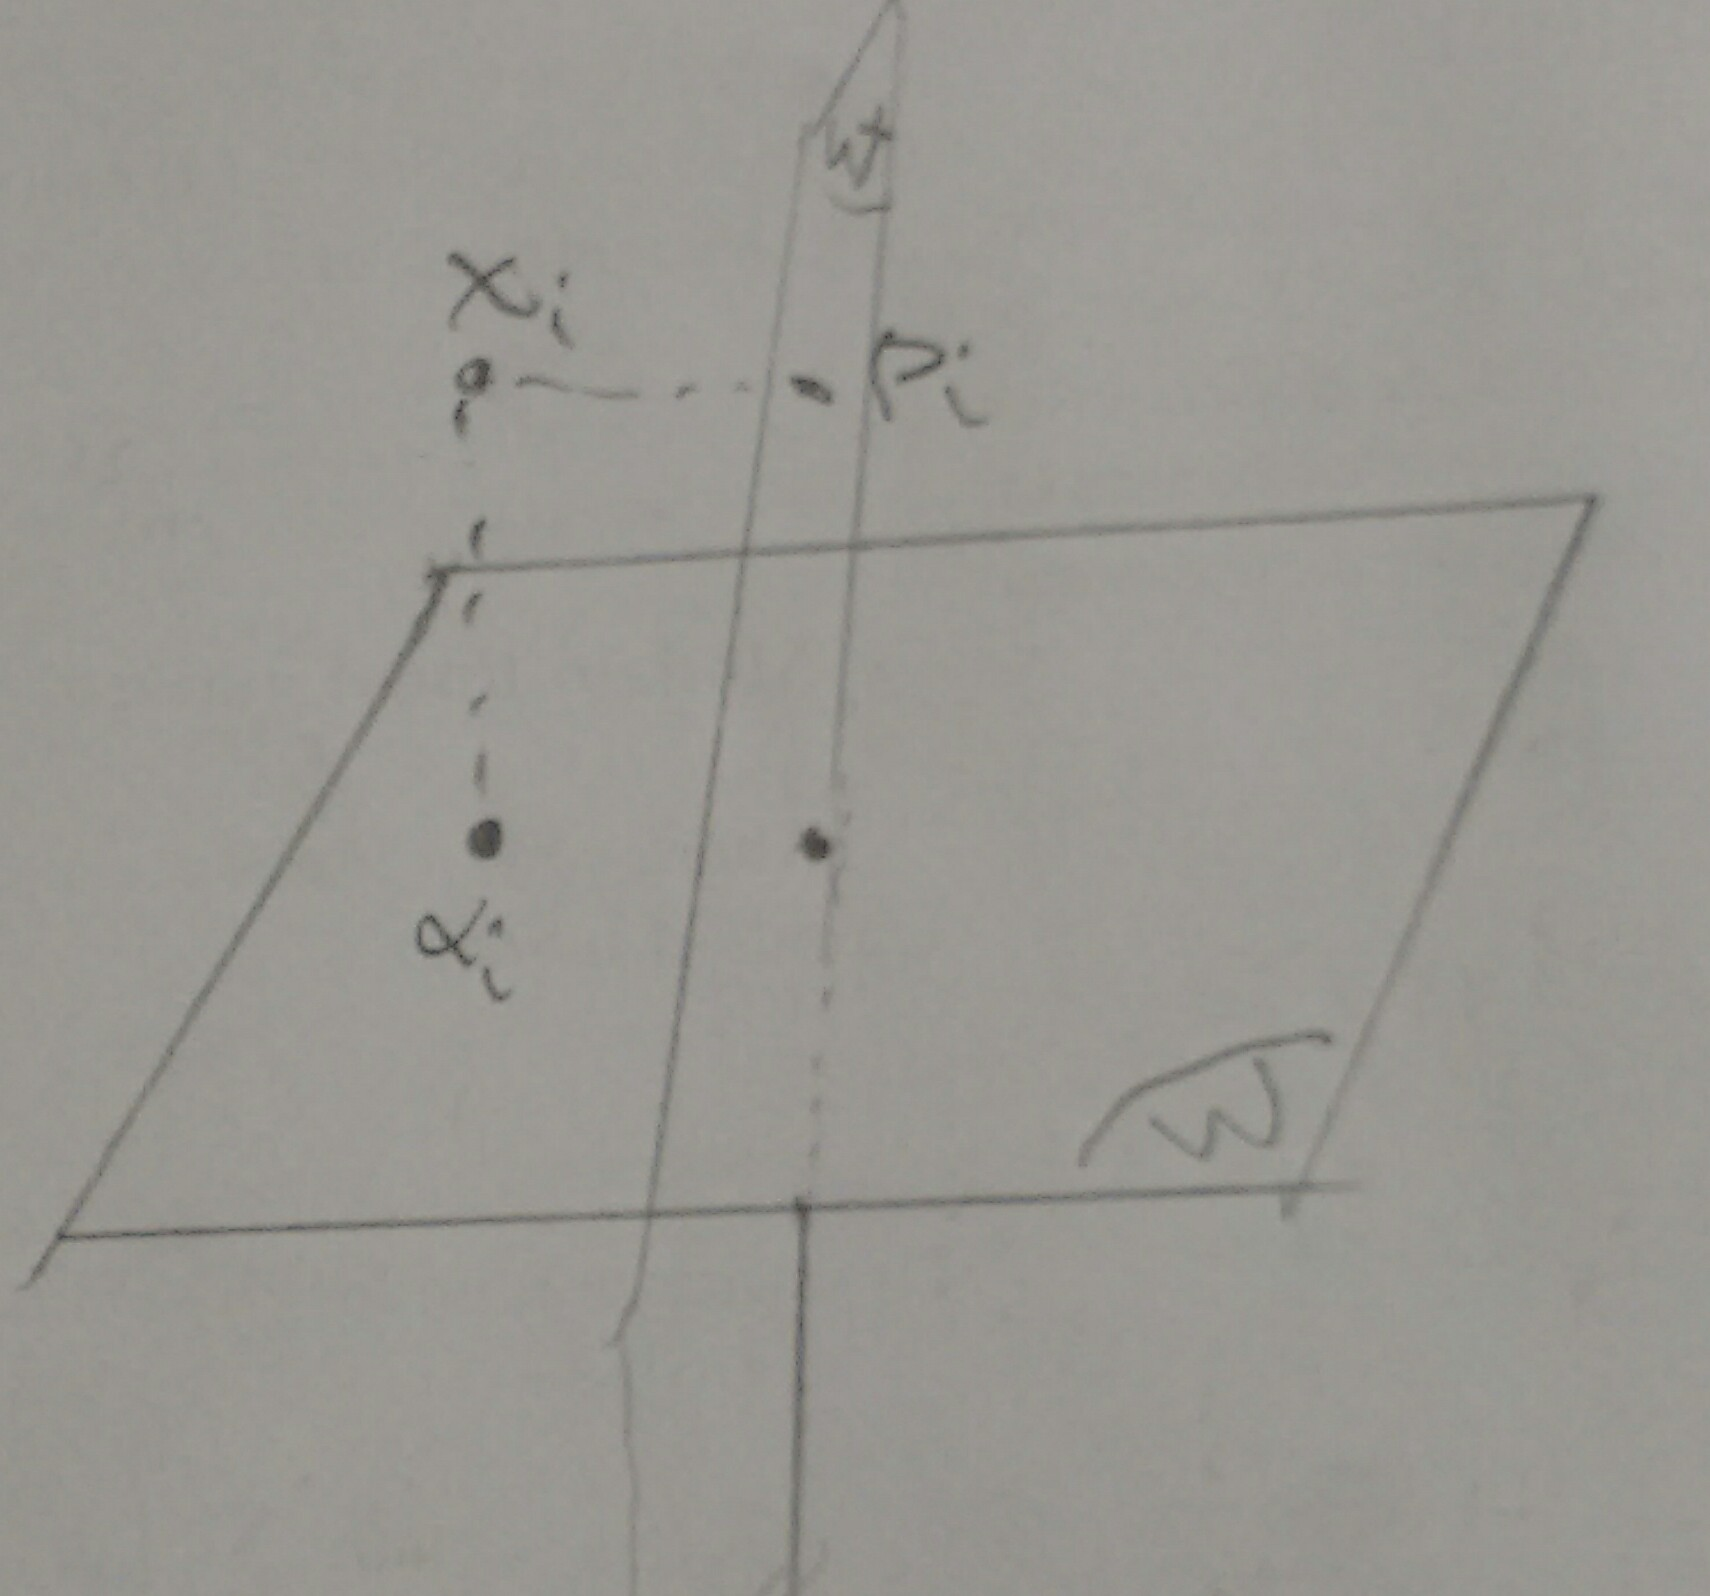
\includegraphics[scale=0.1]{imagenes/descomposicionlineal.jpg}
\end{center}
Se define la inercia de $\mathcal{M}$ con respecto a $W$ como
\begin{align*}
I_{W} = \sum_{i \in I} p_{i}||\beta_{i}||^2
\end{align*}
Análogamente
\begin{align*}
I_{W^{\perp}} \sum_{i \in I} p_{i}||\alpha_{i}||^2
\end{align*}

Por pitágoras $||\alpha_{i}||^2 + ||\beta_{i}||^2 = ||x_{i}||^2$ de modo que
\begin{align*}
\sum p_{i} ||x_{i}||^2 = \sum p_{i}||\alpha_{i}||^2 + \sum p_{i} ||\beta_{i}||^2\\
I_{0} = I_{W} + I_{W^{\perp}}
\end{align*}

¿Qué pasa si $I_{W} = 0$?\\

Esto significa que $||\beta_{i}||^2 = 0, i \in I \Rightarrow \mathcal{M} \subseteq W$
\begin{center}
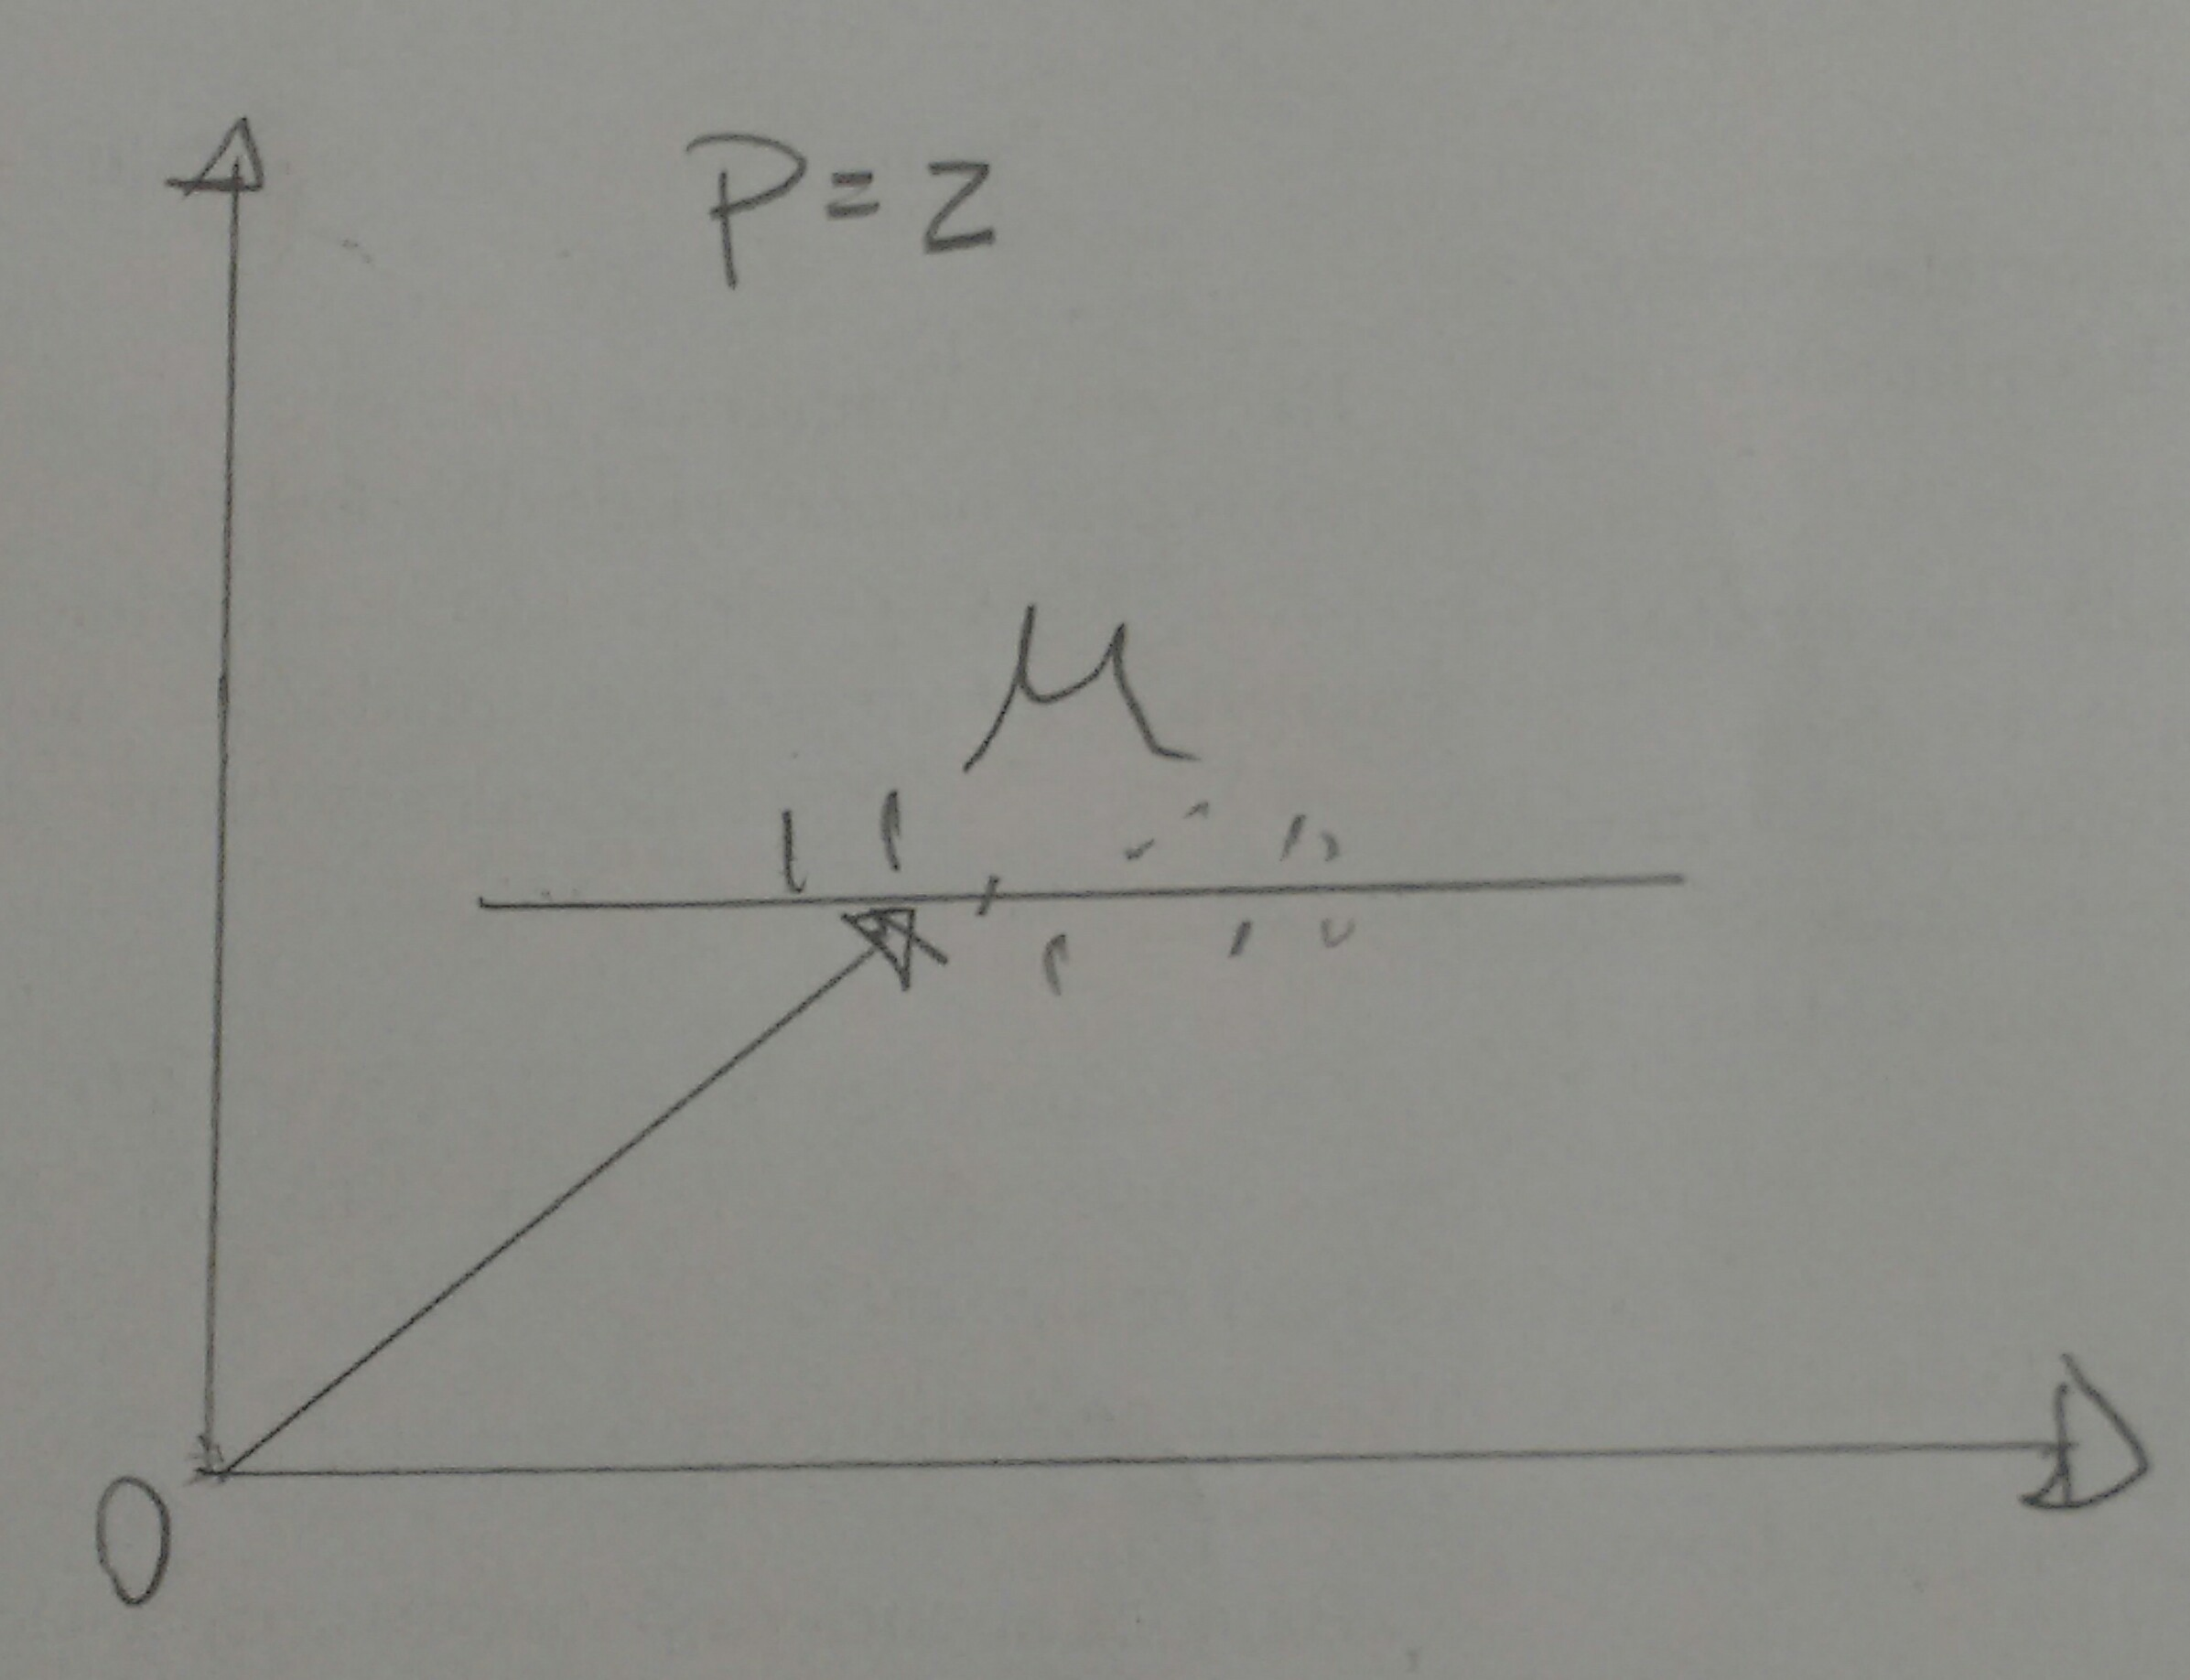
\includegraphics[scale=0.1]{imagenes/afin.jpg}
\end{center}

Inercia con respecto a subespacio vectorial afín\\
Sea $W$ un subespacio vectorial y $a \in W^{\perp}$. Sea $W_{a} = W + a$
\begin{center}
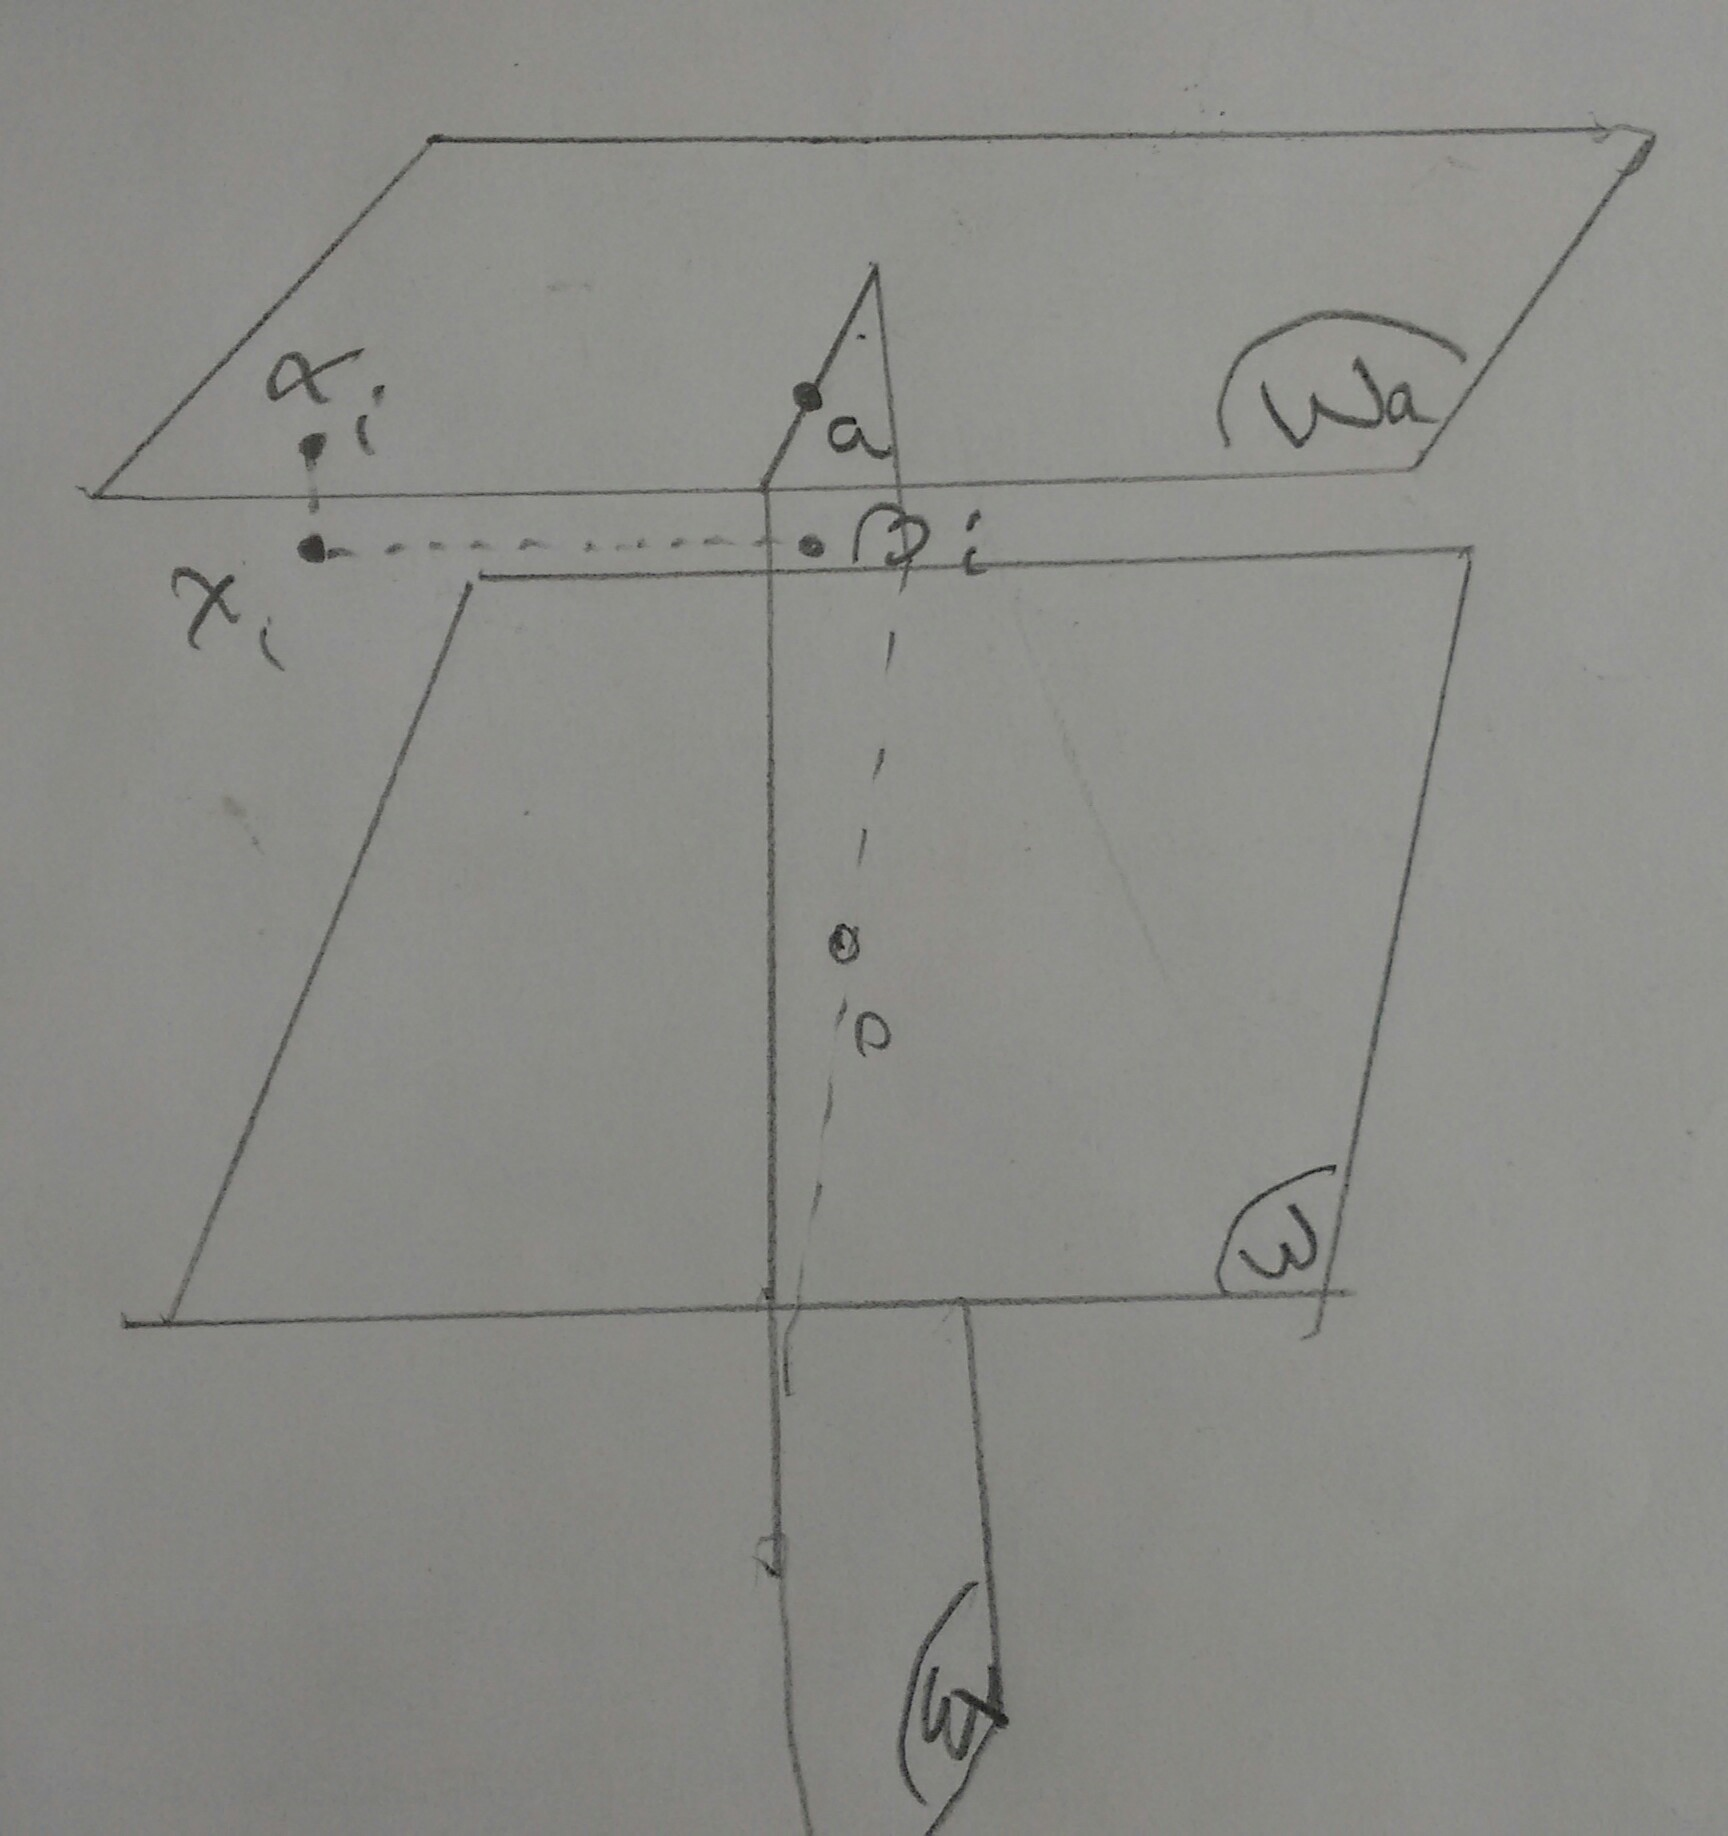
\includegraphics[scale=0.1]{imagenes/descomposicionafin.jpg}
\end{center}

Definimos
\begin{align*}
I_{W_{a}} = \sum_{i \in I} p_{i}||\beta_{i}-a||^2
\end{align*}

Supongamos que nuestra nube es centrada, es decir $g = \sum p_{i}x_{i} = 0$.
\begin{align*}
I_{W_{a}} = \sum p_{i}||\beta_{i}||^2||a||^2 - 2 \sum p_{i} <\beta_{i},a>\\
\sum p_{i}<\beta_{i},a> = <\underline{\sum p_{i}\beta_{i}}_{0}, a>\\
\Rightarrow I_{W_{a}} = I_{W} + ||a||^2
\end{align*}
Es decir, $I_{W_{a}} \ge I_{W} \forall a \in E$, por lo tanto si $g=0$, entonces conviene proyectar siempre en un subespacio vectorial (no afín, que contenga al 0).\\

Dicho de otra manera, si la nube no es centrada ($g\not = 0$), entonces conviene proyectar en un subespacio vectorial afín que contenga a $g$.\\

Una relación sencilla\\

Sean $W_{1}, W_{2}$ subespacios vectoriales ortogonales y $W = W_{1} + W_{2}$. Entonces
\begin{align*}
I_{W^{\perp}} = I_{W_{1}} + I_{W_{2}}
\end{align*}
Si $g=0$ entonces
\begin{align*}
I_{g} = I_{W} + I_{W^{\perp}} + I_{W_{1}^{\perp}} + I_{W_{2}^{\perp}}
\end{align*}
Demostración sencilla 
\begin{align*}
x_{i} = \alpha_{i} + \beta_{i} & \quad \alpha_{i} \in W, \beta_{i} \in W^{\perp}\\
\alpha_{i} = \gamma_{i} + \delta_{i} & \quad \gamma_{i} \in W_{1}, \delta_{i} \in W_{2}\\
x_{i} = \gamma_{i} + \delta_{i} + \beta_{i}
\end{align*}
Entonces como $g=0$
\begin{align*}
I_{g} =\sum p_{i} ||x_{i}||^2 = \sum_{W_{1}^{\perp}}  p_{i} ||\gamma_{i}||^2 + \sum_{W_{2}^{\perp}}  p_{i} ||\delta_{i}||^2 + \sum_{W}  p_{i} ||\beta_{i}||^2
\end{align*}

\begin{teo} subespacio vectorial $W_{k+1}$ de dimensión $k+1$ (que minimiza la inercia) contiene un subespacio vectorial $W_{k}$ de dimensión $k$ que minimiza la inercia. Aquí suponemos que $g=0$
\end{teo}

\begin{proof}
Notar que $dim W_{k} = k$ y $dim W_{k}^{\perp} = p-k$ por lo tanto $W_{k}^{\perp} + W_{k+1} = p-k + k + 1 > p$. Por lo tanto, $dim W_{k}^{\perp}\cap W_{k+1} \ge 1$, luego existe $v \not = 0, v \in W_{k}^{\perp} \cap W_{k+1}$.\\

Si designamos por $\Delta v$ el subespacio vectorial engendrado por $v$, tenemos que
\begin{align*}
W_{k+1} = \Delta v + R
\end{align*}
$R$ el ortogonal a $\Delta v$ en $W_{k+1}$.\\

Por otra parte sea $U$ el espacio que se obtiene
\begin{align*}
U = \Delta v + W_{k}
\end{align*}
Notar que $dim(U) = k+1$.\\

Entonces,
\begin{align*}
I_{W_{k+1}} = I_{g} - I_{\Delta v ^{\perp}} - I_{R^{\perp}}
\end{align*}
y tambi+én
\begin{align*}
I_{U} = I_{g} - I_{\Delta v ^{\perp}} - I_{W_{k}^{\perp}}
\end{align*}
$I_{W_{k}}$ es mínima entre todos los espacios de dimensión $k$, o bien $I_{W_{k}^{\perp}}$ máxima. Por lo tanto,
\begin{align*}
I_{W_{k}^{\perp}} \ge I_{R^{\perp}}\\
\Rightarrow I_{U} \le I_{W_{k+1}}
\end{align*}
Pero por hipótesos $W_{k+1}$ es óptimo, es decir $I_{W_{k+1}} \le I_{U}$. Entonces llegamos a la conclusión $I_{W_{k+1}} = I_{U}$, por lo que $I_{R} = I_{W_{k}}$.\\

Hemos construído un subespacio vectorial $R$ óptimo de dimensión $k$, contenido en $W_{k+1}$.\\

El paso de  $R$ a $W_{k+1}$ se hace agregando un eje $\Delta v$ de mínima inercia.
\end{proof}

\end{document}
